\documentclass[11pt,a4paper]{article}
\usepackage[margin=2.5cm]{geometry}
\usepackage{amsmath,amssymb,amsthm}
\usepackage{booktabs}
\usepackage{microtype}
\usepackage{xcolor}
\usepackage{tikz}
\definecolor{cA}{HTML}{1F4E8C}
\definecolor{cB}{HTML}{B3261E}
\definecolor{cC}{HTML}{1B7A3D}
\definecolor{cD}{HTML}{B36B00}
\newcommand{\blk}[2]{\texttt{\textbf{\textcolor{#1}{#2}}}}
\newcommand{\slide}[4]{\texttt{\textcolor{black!25}{#1}\textbf{\textcolor{#4}{#2}}\textcolor{black!25}{#3}}}
\newcommand{\seq}[1]{\texttt{\small #1}}
\usepackage{parskip}

\theoremstyle{definition}
\newtheorem{definition}{Definition}
\theoremstyle{plain}
\newtheorem{theorem}[definition]{Theorem}

\title{Sturmian sequences of $\sqrt n$}
\author{Robin Langer}
\date{}

\begin{document}
\maketitle
\vspace{-2em}

\section{The window count}

Consider the sequence generated by replacing every $1$ by $10$ and every $0$ by
$1$. Start at $1$ and repeat:
\[
  1, \quad 10, \quad 101, \quad 10110, \quad 10110101, \quad
  1011010110110, \quad \ldots
\]
The limit is the \emph{Fibonacci sequence}
\[
  \ell \;=\; 1\,0\,1\,1\,0\,1\,0\,1\,1\,0\,1\,1\,0\,1\,0\,1 \cdots
\]
Slide a window $m$ letters wide along it and write down every distinct block.
Let $F(m)$ be how many there are. For $m = 3$:

\begin{center}
\begin{tabular}{llll}
\toprule
position & window & block & \\ \midrule
$0$ & \slide{}{101}{1010110110101}{cA} & \blk{cA}{101} & new \\
$1$ & \slide{1}{011}{010110110101}{cB} & \blk{cB}{011} & new \\
$2$ & \slide{10}{110}{10110110101}{cC} & \blk{cC}{110} & new \\
$3$ & \slide{101}{101}{0110110101}{cA} & \blk{cA}{101} & seen \\
$4$ & \slide{1011}{010}{110110101}{cD} & \blk{cD}{010} & new \\
$5$ & \slide{10110}{101}{10110101}{cA} & \blk{cA}{101} & seen \\
$6$ & \slide{101101}{011}{0110101}{cB} & \blk{cB}{011} & seen \\
$7$ & \slide{1011010}{110}{110101}{cC} & \blk{cC}{110} & seen \\
$8$ & \slide{10110101}{101}{10101}{cA} & \blk{cA}{101} & seen \\
\multicolumn{4}{c}{$\cdots$ and nothing new appears after that $\cdots$} \\
\bottomrule
\end{tabular}
\end{center}

Four distinct blocks, so $F(3) = 4$.

\begin{definition}
A sequence is \emph{Sturmian} when $F(m) = m+1$ for every $m \geq 1$.
\end{definition}

The Fibonacci sequence is Sturmian.


\clearpage
\section{Morse and Hedlund}

There is an alternative way to characterize Sturmian sequences.

\begin{center}
\colorbox{black!8}{%
\begin{minipage}{0.93\textwidth}
\begin{theorem}[Morse and Hedlund]
A sequence is Sturmian if and only if there is an irrational $\alpha \in (0,1)$
and a $\rho \in [0,1)$ with
\[
  \ell_k \;=\; \lfloor (k+1)\alpha + \rho \rfloor - \lfloor k\alpha + \rho \rfloor .
\]
\end{theorem}
\end{minipage}}
\end{center}

The formula counts integer crossings. Walk along the real line in steps of
$\alpha$, so that after $k$ steps you stand at position $k\alpha + \rho$. Each step is shorter than a
whole unit, so it passes through at most one integer. We record $\ell_k = 1$ when the
step from $k$ to $k+1$ passes an integer and $\ell_k = 0$ otherwise.

The equivalence of these two definitions is not obvious.

After $k$ steps you have travelled a distance of $k\alpha$. So about $k\alpha$
of the first $k$ letters are $1$s, and the proportion of $1$s is $\alpha$. We call this
both the density and the slope. The second number $\rho$ tells us only where
we start reading the sequence.

\begin{center}
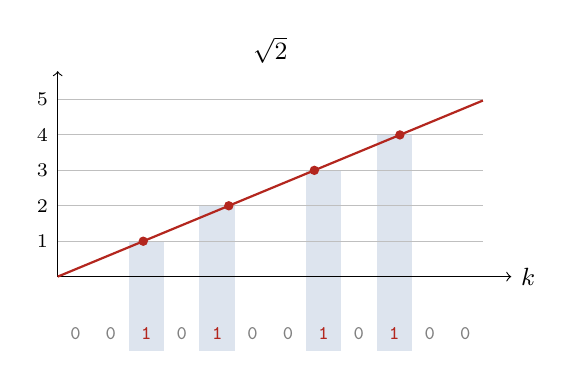
\begin{tikzpicture}[x=0.45cm,y=0.45cm,baseline=0pt]
  \fill[cA!15] (2,-2.1) rectangle (3,1);
  \fill[cA!15] (4,-2.1) rectangle (5,2);
  \fill[cA!15] (7,-2.1) rectangle (8,3);
  \fill[cA!15] (9,-2.1) rectangle (10,4);
  \draw[black!25] (0,1) -- (12,1);
  \draw[black!25] (0,2) -- (12,2);
  \draw[black!25] (0,3) -- (12,3);
  \draw[black!25] (0,4) -- (12,4);
  \draw[black!25] (0,5) -- (12,5);
  \draw[->] (0,0) -- (12.8,0) node[right,font=\small]{$k$};
  \draw[->] (0,0) -- (0,5.8);
  \node[left,font=\scriptsize] at (0,1) {1};
  \node[left,font=\scriptsize] at (0,2) {2};
  \node[left,font=\scriptsize] at (0,3) {3};
  \node[left,font=\scriptsize] at (0,4) {4};
  \node[left,font=\scriptsize] at (0,5) {5};
  \draw[cB,thick] (0,0) -- (12,4.9706);
  \fill[cB] (2.4142,1) circle (1.7pt);
  \fill[cB] (4.8284,2) circle (1.7pt);
  \fill[cB] (7.2426,3) circle (1.7pt);
  \fill[cB] (9.6569,4) circle (1.7pt);
  \node[font=\ttfamily\scriptsize,text=black!50] at (0.5,-1.6) {0};
  \node[font=\ttfamily\scriptsize,text=black!50] at (1.5,-1.6) {0};
  \node[font=\ttfamily\scriptsize\bfseries,text=cB] at (2.5,-1.6) {1};
  \node[font=\ttfamily\scriptsize,text=black!50] at (3.5,-1.6) {0};
  \node[font=\ttfamily\scriptsize\bfseries,text=cB] at (4.5,-1.6) {1};
  \node[font=\ttfamily\scriptsize,text=black!50] at (5.5,-1.6) {0};
  \node[font=\ttfamily\scriptsize,text=black!50] at (6.5,-1.6) {0};
  \node[font=\ttfamily\scriptsize\bfseries,text=cB] at (7.5,-1.6) {1};
  \node[font=\ttfamily\scriptsize,text=black!50] at (8.5,-1.6) {0};
  \node[font=\ttfamily\scriptsize\bfseries,text=cB] at (9.5,-1.6) {1};
  \node[font=\ttfamily\scriptsize,text=black!50] at (10.5,-1.6) {0};
  \node[font=\ttfamily\scriptsize,text=black!50] at (11.5,-1.6) {0};
  \node[font=\small] at (6.0,6.4) {$\sqrt{2}$};
\end{tikzpicture}
\hspace{2em}
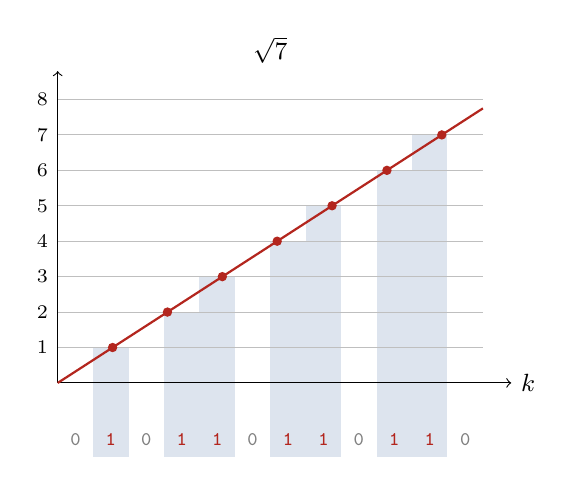
\begin{tikzpicture}[x=0.45cm,y=0.45cm,baseline=0pt]
  \fill[cA!15] (1,-2.1) rectangle (2,1);
  \fill[cA!15] (3,-2.1) rectangle (4,2);
  \fill[cA!15] (4,-2.1) rectangle (5,3);
  \fill[cA!15] (6,-2.1) rectangle (7,4);
  \fill[cA!15] (7,-2.1) rectangle (8,5);
  \fill[cA!15] (9,-2.1) rectangle (10,6);
  \fill[cA!15] (10,-2.1) rectangle (11,7);
  \draw[black!25] (0,1) -- (12,1);
  \draw[black!25] (0,2) -- (12,2);
  \draw[black!25] (0,3) -- (12,3);
  \draw[black!25] (0,4) -- (12,4);
  \draw[black!25] (0,5) -- (12,5);
  \draw[black!25] (0,6) -- (12,6);
  \draw[black!25] (0,7) -- (12,7);
  \draw[black!25] (0,8) -- (12,8);
  \draw[->] (0,0) -- (12.8,0) node[right,font=\small]{$k$};
  \draw[->] (0,0) -- (0,8.8);
  \node[left,font=\scriptsize] at (0,1) {1};
  \node[left,font=\scriptsize] at (0,2) {2};
  \node[left,font=\scriptsize] at (0,3) {3};
  \node[left,font=\scriptsize] at (0,4) {4};
  \node[left,font=\scriptsize] at (0,5) {5};
  \node[left,font=\scriptsize] at (0,6) {6};
  \node[left,font=\scriptsize] at (0,7) {7};
  \node[left,font=\scriptsize] at (0,8) {8};
  \draw[cB,thick] (0,0) -- (12,7.7490);
  \fill[cB] (1.5486,1) circle (1.7pt);
  \fill[cB] (3.0972,2) circle (1.7pt);
  \fill[cB] (4.6458,3) circle (1.7pt);
  \fill[cB] (6.1943,4) circle (1.7pt);
  \fill[cB] (7.7429,5) circle (1.7pt);
  \fill[cB] (9.2915,6) circle (1.7pt);
  \fill[cB] (10.8401,7) circle (1.7pt);
  \node[font=\ttfamily\scriptsize,text=black!50] at (0.5,-1.6) {0};
  \node[font=\ttfamily\scriptsize\bfseries,text=cB] at (1.5,-1.6) {1};
  \node[font=\ttfamily\scriptsize,text=black!50] at (2.5,-1.6) {0};
  \node[font=\ttfamily\scriptsize\bfseries,text=cB] at (3.5,-1.6) {1};
  \node[font=\ttfamily\scriptsize\bfseries,text=cB] at (4.5,-1.6) {1};
  \node[font=\ttfamily\scriptsize,text=black!50] at (5.5,-1.6) {0};
  \node[font=\ttfamily\scriptsize\bfseries,text=cB] at (6.5,-1.6) {1};
  \node[font=\ttfamily\scriptsize\bfseries,text=cB] at (7.5,-1.6) {1};
  \node[font=\ttfamily\scriptsize,text=black!50] at (8.5,-1.6) {0};
  \node[font=\ttfamily\scriptsize\bfseries,text=cB] at (9.5,-1.6) {1};
  \node[font=\ttfamily\scriptsize\bfseries,text=cB] at (10.5,-1.6) {1};
  \node[font=\ttfamily\scriptsize,text=black!50] at (11.5,-1.6) {0};
  \node[font=\small] at (6.0,9.4) {$\sqrt{7}$};
\end{tikzpicture}
\end{center}

\clearpage
\section{The sequence of a square root}

Put $a_0 = \lfloor \sqrt n \rfloor$ and take the slope to be
\[
  \alpha \;=\; \sqrt n - a_0 ,
  \qquad
  \ell_k \;=\; \lfloor (k+1)\alpha \rfloor - \lfloor k\alpha \rfloor .
\]
If $\sqrt n = [\,a_0;\ \overline{a_1, \ldots, a_L}\,]$ then
$\alpha = [\,0;\ \overline{a_1, \ldots, a_L}\,]$, periodic from $a_1$.

$\alpha = [\,0;\, a_1, a_2, a_3, \ldots\,]$ means $\alpha = 1/(a_1 + \beta)$
with $\beta = [\,0;\, a_2, a_3, \ldots\,]$, so
\[
  \frac{1}{\alpha} \;=\; a_1 + \beta ,
  \qquad
  \beta \in (0,1) .
\]
From which it follows that:
\[
  a_1 \alpha \;<\; 1 \;<\; (a_1 + 1)\alpha .
\]
The next $1$ therefore comes after $a_1$ or $a_1 + 1$ steps, and the number of
consecutive $0$s between any two consecutive $1$s must be $a_1 - 1$ or $a_1$.

We define a new sequence $\ell'$, the \emph{derived sequence}, by setting
\[
  \ell'_k \;=\;
  \begin{cases}
    1 & \text{if $a_1$ zeros lie between the $k$th and $(k{+}1)$th $1$ of $\ell$},\\
    0 & \text{if $a_1 - 1$ do}.
  \end{cases}
\]

\section{$n = 2$}

$\sqrt 2 = [\,1;\ \overline{2}\,]$, so $L = 1$ and
$\alpha = \sqrt 2 - 1$.
\[
  \ell \;=\; \seq{\textcolor{black!45}{00}\textcolor{cA}{10}\textcolor{cB}{100}\textcolor{cA}{10}\textcolor{cB}{100}\textcolor{cA}{10}\textcolor{cA}{10}\textcolor{cB}{100}\textcolor{cA}{10}\textcolor{cB}{100}\textcolor{cA}{10}\textcolor{cA}{10}\textcolor{cB}{100}\textcolor{cA}{10}\textcolor{cB}{100}\textcolor{cA}{10}\textcolor{cB}{100}\textcolor{cA}{10}}\cdots
\]
The $1$s sit at
\[
  2,\ 4,\ 7,\ 9,\ 12,\ 14,\ 16,\ 19,\ 21,\ 24,\ 26,\ 28,\ 31,\ 33, \ \ldots
\]
and the numbers of $0$s between them are
\[
  1,\ 2,\ 1,\ 2,\ 1,\ 1,\ 2,\ 1,\ 2,\ 1,\ 1,\ 2,\ 1,\ 2, \ \ldots
\]
The derived sequence is thus:
\[
  \ell' \;=\; \seq{\textcolor{cA}{0}\textcolor{cB}{1}\textcolor{cA}{0}\textcolor{cB}{1}\textcolor{cA}{0}\textcolor{cA}{0}\textcolor{cB}{1}\textcolor{cA}{0}\textcolor{cB}{1}\textcolor{cA}{0}\textcolor{cA}{0}\textcolor{cB}{1}\textcolor{cA}{0}\textcolor{cB}{1}\textcolor{cA}{0}\textcolor{cB}{1}\textcolor{cA}{0}}\cdots
\]
Observe that the derived sequence is the original sequence with the first letter
removed.

Here
\[
  \frac{1}{\alpha} \;=\; \sqrt 2 + 1 \;=\; 2 + \beta ,
  \qquad
  \beta \;=\; \sqrt 2 - 1 \;=\; \alpha ,
\]

\clearpage
\section{$n = 7$}

$\sqrt 7 = [\,2;\ \overline{1,1,1,4}\,]$, so $L = 4$ and
$\alpha = \sqrt 7 - 2$.
\[
  \ell \;=\; \seq{\textcolor{black!45}{0}\textcolor{cB}{10}\textcolor{cA}{1}\textcolor{cB}{10}\textcolor{cA}{1}\textcolor{cB}{10}\textcolor{cA}{1}\textcolor{cB}{10}\textcolor{cA}{1}\textcolor{cB}{10}\textcolor{cB}{10}\textcolor{cA}{1}\textcolor{cB}{10}\textcolor{cA}{1}\textcolor{cB}{10}\textcolor{cA}{1}\textcolor{cB}{10}\textcolor{cA}{1}\textcolor{cB}{10}\textcolor{cA}{1}\textcolor{cB}{10}\textcolor{cB}{10}\textcolor{cA}{1}\textcolor{cB}{10}\textcolor{cA}{1}\textcolor{cB}{10}\textcolor{cA}{1}\textcolor{cB}{10}\textcolor{cA}{1}}\cdots
\]
The $1$s sit at
\[
  1,\ 3,\ 4,\ 6,\ 7,\ 9,\ 10,\ 12,\ 13,\ 15,\ 17,\ 18,\ 20,\ 21, \ \ldots
\]
and the numbers of $0$s between them are
\[
  1,\ 0,\ 1,\ 0,\ 1,\ 0,\ 1,\ 0,\ 1,\ 1,\ 0,\ 1,\ 0,\ 1, \ \ldots
\]
The blocks are \texttt{1} and \texttt{10}:

\begin{center}
\begin{tabular}{l@{\quad}*{12}{c@{\;\;}}}
\toprule
$\ell$ & \textcolor{black!45}{\seq{0}} & \textcolor{cB}{\seq{10}} & \textcolor{cA}{\seq{1}} & \textcolor{cB}{\seq{10}} & \textcolor{cA}{\seq{1}} & \textcolor{cB}{\seq{10}} & \textcolor{cA}{\seq{1}} & \textcolor{cB}{\seq{10}} & \textcolor{cA}{\seq{1}} & \textcolor{cB}{\seq{10}} & \textcolor{cB}{\seq{10}} & \textcolor{cA}{\seq{1}} \\
$\ell'$ &  & \textcolor{cB}{\seq{1}} & \textcolor{cA}{\seq{0}} & \textcolor{cB}{\seq{1}} & \textcolor{cA}{\seq{0}} & \textcolor{cB}{\seq{1}} & \textcolor{cA}{\seq{0}} & \textcolor{cB}{\seq{1}} & \textcolor{cA}{\seq{0}} & \textcolor{cB}{\seq{1}} & \textcolor{cB}{\seq{1}} & \textcolor{cA}{\seq{0}} \\
\bottomrule
\end{tabular}
\end{center}

Four derivations run through the period:

\begin{center}
\begin{tabular}{llll}
\toprule
 & $\alpha$ & & sequence \\ \midrule
$\ell$      & $\sqrt 7 - 2$        & $[\,0;\,\overline{1,1,1,4}\,]$ & \seq{01011011011011010110110110110110} \\
derive      & $(\sqrt 7 - 1)/3$    & $[\,0;\,\overline{1,1,4,1}\,]$ & \seq{10101010110101010101101010101101} \\
derive$^2$  & $(\sqrt 7 - 1)/2$    & $[\,0;\,\overline{1,4,1,1}\,]$ & \seq{11110111110111101111101111101111} \\
derive$^3$  & $(\sqrt 7 - 2)/3$    & $[\,0;\,\overline{4,1,1,1}\,]$ & \seq{00010000100010000100001000100001} \\
derive$^4$  & $\sqrt 7 - 2$        & $[\,0;\,\overline{1,1,1,4}\,]$ & \seq{10110110110110101101101101101101} \\
\bottomrule
\end{tabular}
\end{center}

The last row is $\ell$ shifted one letter. Every sequence in the table is
Sturmian.

\section{The Fibonacci sequence}

\[
  \ell \;=\; \seq{10110101101101011010110110101101101011010110}\cdots
\]
The $1$s sit at
\[
  0,\ 2,\ 3,\ 5,\ 7,\ 8,\ 10,\ 11,\ 13,\ 15,\ 16,\ 18,\ 20,\ 21, \ \ldots
\]
and the numbers of $0$s between them are
\[
  1,\ 0,\ 1,\ 1,\ 0,\ 1,\ 0,\ 1,\ 1,\ 0,\ 1,\ 1,\ 0,\ 1, \ \ldots
\]
The blocks are \texttt{1} and \texttt{10}:

\begin{center}
\begin{tabular}{l@{\quad}*{12}{c@{\;\;}}}
\toprule
$\ell$ & \textcolor{cB}{\seq{10}} & \textcolor{cA}{\seq{1}} & \textcolor{cB}{\seq{10}} & \textcolor{cB}{\seq{10}} & \textcolor{cA}{\seq{1}} & \textcolor{cB}{\seq{10}} & \textcolor{cA}{\seq{1}} & \textcolor{cB}{\seq{10}} & \textcolor{cB}{\seq{10}} & \textcolor{cA}{\seq{1}} & \textcolor{cB}{\seq{10}} & \textcolor{cB}{\seq{10}} \\
$\ell'$ & \textcolor{cB}{\seq{1}} & \textcolor{cA}{\seq{0}} & \textcolor{cB}{\seq{1}} & \textcolor{cB}{\seq{1}} & \textcolor{cA}{\seq{0}} & \textcolor{cB}{\seq{1}} & \textcolor{cA}{\seq{0}} & \textcolor{cB}{\seq{1}} & \textcolor{cB}{\seq{1}} & \textcolor{cA}{\seq{0}} & \textcolor{cB}{\seq{1}} & \textcolor{cB}{\seq{1}} \\
\bottomrule
\end{tabular}
\end{center}

Observe that the derived sequence is the original sequence.

Take that as the defining property and solve for $\alpha$. The steps are $1$ and
$2$, so $a_1 = 1$ and $1/\alpha = 1 + \beta$. The derived sequence is $\ell$, so
$\beta = \alpha$ and
\[
  \frac{1}{\alpha} \;=\; 1 + \alpha ,
  \qquad
  \alpha^2 + \alpha - 1 \;=\; 0 ,
  \qquad
  \alpha \;=\; \frac{\sqrt 5 - 1}{2} \;=\; \frac{1}{\varphi} .
\]
The golden mean falls out as the slope of the Fibonacci sequence.

In continued fractions,
\[
  \frac{1}{\varphi} \;=\; [\,0;\, 1, 1, 1, 1, \ldots\,] ,
\]
because $\varphi = 1 + 1/\varphi$. Deriving deletes $a_1$ and leaves the list
unchanged.

\section{Square roots as sequences}

Deriving a Sturmian sequence sends the slope $\alpha$ to $\{1/\alpha\}$, which
deletes the first term $a_1$ of the continued fraction expansion. So the tower
of derived sequences circles back exactly when the continued fraction of
$\alpha$ repeats.

\begin{center}
\colorbox{black!8}{%
\begin{minipage}{0.93\textwidth}
\begin{theorem}[Lagrange]
The continued fraction of $\alpha$ is eventually periodic if and only if
$\alpha$ is a quadratic irrational,
\[
  \alpha \;=\; \frac{a + \sqrt n}{b} ,
\]
with $a$, $b$ and $n$ integers and $n$ not a square.
\end{theorem}
\end{minipage}}
\end{center}

Sturmian sequences with cyclical derived sequences give us another way to
think about quadratic irrationals.

\end{document}

